%%%%%%%%%%%%%%%%%%%%%%%%%%%%%%%%%%%%%%%%%%%%%%%%%%%%%%%%%%%%%%%%%%%%%%%%%%%%%%%%%%
%%% Introduction
%%%%%%%%%%%%%%%%%%%%%%%%%%%%%%%%%%%%%%%%%%%%%%%%%%%%%%%%%%%%%%%%%%%%%%%%%%%%%%%%%%
\chapter{Introduction}
	\label{ch::introduction}

		The design of legged robots and associated methods of locomotion control has been an area of interest spanning the past several decades, as shown by \cite{McGhee1965,Hodgins1991,Altendorfer2001,Kolter2008,Wieber2015}. Quadruped robotic systems have gained popularity in studies pertaining to variable terrain navigation and full-body stability adaptation. Well known examples of this from the past 15 years are the Tekken \cite{Fukuoka2003}, Kolt \cite{Estremera2006}, BigDog \cite{BigDog2008}, and HyQ \cite{Semini2010_PHD} quadrupeds. Many of these systems have been implemented on a larger scale so that they can carry substantial payloads while maintaining adequate system bandwidth for fast gaits and robustness to rough terrains. Few, however, have been implemented on the scale of a hobby-robot platform while still maintaining an aptitude for rough terrain navigation and comparable sensory prowess.

		The BlueFoot quadruped is a self-contained, fully-actuated platform with the dexterity to perform stabilization and repositioning maneuvers on variable terrains along the same lines as the LittleDog platform \cite{Rebula2007}. Namely, BlueFoot has been designed with sixteen actuated degrees of freedom to allow for the execution of a wide range of body and leg articulations. This level of dexterity grants the BlueFoot platform the ability to articulate its trunk over a range of poses, as well as overcome raised or uneven terrain. 

		BlueFoot is outfitted with several on-board vision sensors, including a LIDAR and camera, which are mounted to its trunk (main body). BlueFoot can articulate (\IE pitch and yaw) these sensors by reposing its trunk using aggregate leg motion controls. BlueFoot also includes a sizable array of other on-board sensors for feedback and control, including joint position, velocity and loading sensors; an inertial measurement unit (IMU); and foot-contact sensors. Using the computational, sensory and motor capacities at hand, BlueFoot has the ability to utilize similar control mechanisms to those implemented on larger quadruped systems. 

		The BlueFoot platform inherently demands a variety of control routines to achieve locomotion and system stability, making this robot an ample platform for studies related to gait design and motion planning. In particular, BlueFoot's controllers makes direct use of the system's kinematic model; and involve applications of open-loop gait design and stabilization for the purpose of achieving dynamic locomotion control. In particular, BlueFoot is gaited via a central pattern generator (CPG) based technique which is augmented with a foothold controller along the same lines as \cite{Ajallooeian2013} and \cite{Rutishauser2008}. Active platform stabilization is performed via a zero-moment point (ZMP) based body placement controller which stabilizes the system using planar trunk motions during arbitrary gaiting sequences. Both such controllers make use of virtual-forces to drive system reference commands. These controllers apply BlueFoot's forward kinematic model for the purpose estimating joint and foot positions. Finally, outer-loop control routines are implemented to supply commands and corrections used in system navigation control. Among these controllers are a potential-fields navigation controller, which incorporates image-feature tracking; and 3D point-cloud processing routines for surface reconstruction and foot-placement planning.
	
			\begin{figure}[h!]
				\centering
				\fbox{\includegraphics[width=1.0\textwidth]{on_the_rocks2.jpg}}
				\caption{The BlueFoot Quadruped Robot}
				\label{fig::bluefoot_glamour}
			\end{figure}





	\section{Central Pattern Generators for Gait Control}

		As previously mentioned, BlueFoot's core gaiting routine relies on the utilization of artificial Central Pattern Generators (CPGs). This control mechanism is inspired from biological neural networks which generate rhythmic motions \cite{Ijspeert2008}. \cite{Arena2000} describes biological CPGs as a form of self-organizing cellular neural network, and also explains the role of limited feedback in CPG networks. In fact, a key feature of these networks is that they can act without explicit sensory feedback inputs or directions from a higher-level command unit, such as a brain. Instead, signals emanating from independent motor units (and, sometimes, feedback gathered from sensory neurons) are utilized to trigger or inhibit a sequence of successive, self-coordinated motor operations. These activation sequences create loops which give rise to cyclic motion patterns. 

		In robotics, biological CPG's are modeled via an artificial counterpart which applies multi-state unit-oscillators to represent neural units. The dynamics of each unit oscillator in an artificial CPG network are designed to influence the dynamics of other network oscillators through tunable coupling parameters. Typically, the coupled oscillator network is implemented on a digital controller, which numerically integrates the dynamics of each neural oscillator. The output states of each unit-oscillator are used to drive selected robot degrees of freedom. Oscillator outputs could also be used for planning periodic motions in the robot's task space, which are then translated into the joint-space references via an inverse kinematics mapping, as is done in BlueFoot's gait control routine. In implementation, specific motions are achieved  through careful tuning of oscillator coupling parameters which incurs particular phase offsets between the individual limit-cycles produced by each unit-oscillator. The ability to coordinate unit-oscillator dynamics is what allows artificial CPGs to be used in the control of higher-level motor tasks, such as walking or crawling.

		The selection of a unit-oscillator for use in a CPG network is a fundamental matter in CPG network design. CPG networks can be designed to employ unit-oscillators with varying oscillator dynamics (\IE varying number of states, tuning parameters, etc.) which exhibit different limit-cycle behaviors. Hopf Oscillators are used in BlueFoot's CPG implementation, as well as in \cite{Righetti2006,Rutishauser2008,Matos2010}. Other unit-oscillator types which have been applied to CPGs include Van der Poll Oscillators, as detailed in \cite{Ijspeert2008}, and the Matsuoka Neural Oscillator \cite{Endo2004}.

		Studies dealing specifically the application of CPG's to multi-legged robot gaiting (specifically quadruped, hexapods and octopodal robots) have been carried out by \cite{Arena2001,Klaassen2002,Arena2004,Inagaki2003,Inagaki2006,Billard2000,Brambilla2006,Buchli2006,Tsujita2001,Tsujita2004}.  In particular, \cite{Ijspeert2008} states that the attractiveness of CPG's in the control of legged robot locomotion lies in the ability to decouple robot motor control, \IE walking, from higher-level planning, such as navigation and body-posture control. Additionally, CPG's offer an effective way for smoothly switching between gaiting patterns, such as walking, trotting, or pacing, simply through the modification of a few control parameters. Moreover, the application of artificial CPG's greatly reduces the dimensionality of the gaiting control problem for legged robots.

		The specific CPG controller implemented on the BlueFoot robot allows for the generation of coordinated motions which can be modified to yield different overall motion patterns without explicitly directing the motion each joint. Moreover, BlueFoots CPG controller does not use a separate unit-oscillator to control the motion of each joint. Instead, four unit-oscillators are used to control the motion of each \emph{foot}. In doing so, CPG outputs are mapped to stepping trajectories in the robot task-space. The resulting task-space reference commands are mapped into angular joint position references using an inverse kinematics solution for the entire robot. This approach gives way to a hybrid gaiting mechanism which combines the conveniences of CPG-based gaiting with the explicitness of strict foot trajectory planning. In BlueFoot's control scheme, foot-placement is prescribed via a separate planning mechanism which is entirely decoupled from the CPG gait controller. This controller hybridization allows a CPG-based motion generator to be applied to gaiting over varying terrains.

		Another important aspect of BlueFoot's CPG implementation is the incorporation of feedback mechanisms which modify CPG parameters. The use of feedback towards improving gaiting stability in CPG-based applications was inspired by the work of \cite{Fukuoka2003,Endo2004}. Namely, BlueFoot's CPG-based gait generation incorporates inertial feedback signals into its CPG mechanism by using them to modify unit-oscillator amplitudes and modulate unit-oscillator frequencies. Coupling the unit-oscillator dynamics with sensory feedback gives rise \emph{reflexive} motions which can be tuned to help prevent the system from excessive tipping during gaiting. Reflexive motion incorporation, as it is applied into BlueFoot's CPG gaiting scheme, will be covered in more detail in Section~\ref{sec::cpg_gait_control}.

		Because CPG-based gaits are inherently open-loop motion control routines, a combination of auxiliary mechanisms must be used in concert with the CPG gait controller in order to ensure system stability during gaiting. The incorporation of feedback signals to modify CPG parameters aids in achieving this to some degree, but is usually insufficient for stable walking over largely uneven terrains.  Additionally, this method requires very careful parametric tuning to work robustly under a larger variety of terrain conditions. Thus, other means of stabilization have been incorporated into BlueFoot's gaiting routine to aid in stability. 

		BlueFoot's core stabilization routine applies a concept named \emph{artificial synergy synthesis}. Using this technique, gait control is carried out independently of a stabilization control. Namely, body stabilization is performed by a subset of the robot's degrees of freedom while gaiting is carried out by the remaining \cite{Vuko1972,Yamaguchi1993}. In original implementations of this technique, adaptations to trunk motion were utilized to stabilize the overall motion of the robot utilizing a ZMP-based approach while gaiting is controlled by a fixed-motion routine. Here, body and foot-placement are both controlled as independent, dynamic routines which supply reference commands in the robot task-space. %These commands are combined using the robot's inverse kinematics solution, which generates a final set of angular position references, which are used to control servo motors at each joint.




	\section{Zero Moment Point Body Placement Control}

		The zero-moment point (ZMP), which is equivalent to the center of pressure (CoP), is formally defined as a point on the ground beneath a walking system at which the net moment acting upon the trunk (referred to as the \emph{tipping moment}) is zero \cite{Sardain2004}. The concept of ZMP and its application to legged robotics was originally introduced by \cite{Vuko1972} and expanded upon in \cite{Goswami1999}. Both such studies apply ZMP theory towards the control of biped robots.

		Formally, the ZMP, denoted $p_{ZMP}$, can be defined using a formulation for the CoP wherein the moments about $\tau_{x}$ and $\tau_{y}$, the lateral tipping-moments applied to the robot's body in the world frame, are equal to zero. The solution for $p_{ZMP}\in\Re^{3}$, with respect to a set of $N$ foot contact points $p_{i,e}\in\Re^{3}$ and $N$ associated applied foot-contact forces $f_{i,e}\in\Re^{3}$, arises as a bounded set of solutions to the equation
			\begin{equation}
				\sum^{N}_{i=1}\wrap{p_{i,e}-p_{ZMP}}\times f_{i,e} 
				= 
				\left[
					\begin{array}{c}
						\tau_{x}	\\
						\tau_{y}	\\
						\tau_{z}
					\end{array}
				\right]
				=
				\left[
					\begin{array}{c}
						0			\\
						0			\\
						*
					\end{array}
				\right]
			\end{equation}
		where $z$-coordinate of $p_{ZMP}$, $\zcomp{p_{ZMP}}$, is strictly zero when the walking surface is flat, as shown in \cite{Wieber2015}. Here, derivations for flat-surface ZMP motion will be described, but equations associated with this technique can be extended to non-flat terrain motion in a straight-forward way with a conceptually equivalent end result. The following expression is derived from dynamical equations which describe the total angular momentum, $\dot{L}$, about the legged system's center of gravity (COG), $p_{COG}$:
			\begin{equation}
				\dot{L} = \sum_{i=1}^{N} p_{i,e}\times f_{i,e} - m_{T} p_{COG} \times \wrap{ \ddot{p}_{COG} + \vec{g} }
			\end{equation}
		where $m_{T}$ is the total mass of the legged system and $\vec{g}$ is the standard gravity vector. Assuming that all points of foot-contacts exist on a flat plane, \IE $\zcomp{p_{i,e}}=0\SSep \forall i=\{1,...,N\}$, and all contact force, $f_{i,e}$ are pointing upward, the $p_{ZMP}$ of the system can be written as
			\begin{equation}
				p_{ZMP} 
				= 
				\frac{ \sum_{i=1}^{N} \wrap{ p_{i,e} \times f_{i,e} } }{ \sbrack{\sum_{i=1}^{N} f_{i,e}}_{z} }
				= 
				\frac{ 	p_{COG} \times \wrap{ \ddot{p}_{COG} + \vec{g} } + \dot{L}m_{T}^{-1} }{ \zcomp{ \ddot{p}_{COG} + \vec{g} }}
				\in \mmathcal{C}_{ZMP} 
			\end{equation}
		where
			\begin{equation}
				\mmathcal{C}_{ZMP} = \convhull{p_{1,e},p_{2,e}...,p_{N,e}}
			\end{equation}
		with $\text{conv}(*)$ defining a convex hull generated from a set of input points, $(*)$. $\mmathcal{C}_{ZMP}$ is used to represent the solution space of $p_{ZMP}$. Moreover, $\mmathcal{C}_{ZMP}$ places a bound on the angular momentum $\dot{L}$ which results from contact variations presented through $p_{i,e}$ and $f_{i,e}$. Setting $\dot{L}=0$, a condition is defined for zero tipping. For BlueFoot's ZMP controller formulation, it is also assumed that the acceleration of the COG is sufficiently small, \IE $\ddot{p}_{COG}\approx0$ which yields the following, intuitive condition for minimal tipping:
			\begin{equation}
				\norm{p_{ZMP} - p_{COG}} < \epsilon
			\end{equation}
		where $\epsilon$ is a scalar bounding constant used to ensure $p_{COG}$ also falls within the bounded set $\mmathcal{C}_{ZMP}$. Thus, the general idea of this ZMP-based controller is to compute an approximate ZMP location and place the center of the robot's trunk (described by the translation $p_{b}$) such that the platform's COG approaches its associated ZMP for some arbitrary kinematic configuration. This is done in an effort to reduce $\norm{\dot{L}}$, so as to avoid tipping about the contacting feet.







	\section{Trunk stabilization}

		In addition to the aforementioned task-space controllers, a learning controller, which features the use of a NARX neural network (NARN-NN), has been studied and evaluated. In essence, this controller learns to approximate disturbance dynamics during periodic gait routines and corrects trunk orientation by administering adaptations to joint position controls. The goal of this NARX-NN based control routine is to achieve a level trunk during locomotion.
		
			\begin{figure}[h!]
				\centering
				\fbox{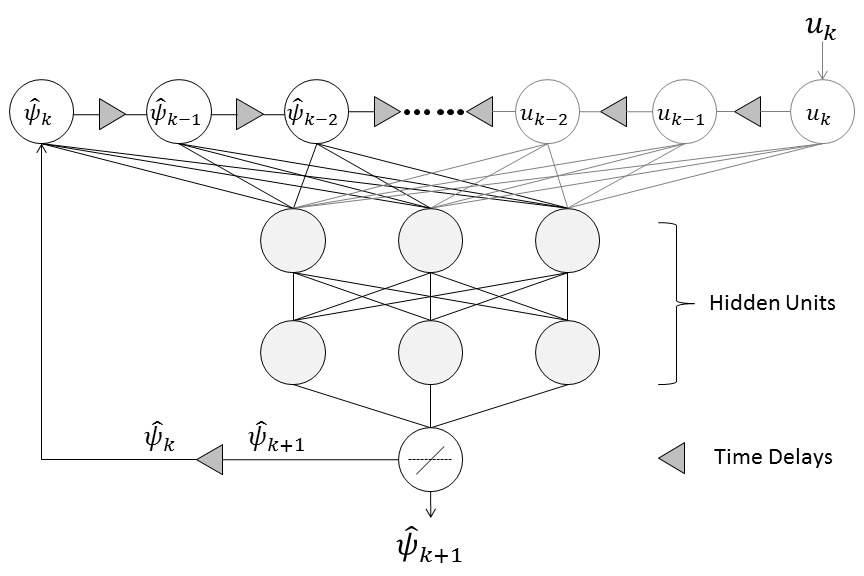
\includegraphics[width=1.0\textwidth]{narx_network_diagram.png}}
				\caption{Parallel NARX-network model with a linear output layer.}
				\label{fig::narx_net}
			\end{figure}

		A NARX-NN architecture is used in this controller because of  its known effectiveness in approximating nonlinear difference systems and making multivariate time-series predictions \cite{Tsungnan1996,ChenBillings1990,Hihi1996,Billings2013}. Moreover, the NARX-NN is a natural fit for a problem of this nature where the dynamics being considered are both periodic and of a high enough complexity where a nonlinear approximation method is warranted. The parallel NARX-NN model, shown in Figure \ref{fig::narx_net}, is comprised of a feed-forward neural network whose input layer accepts a series of time-delayed system state values and network-output histories. The NARX-NN is trained to predict system states in the next time-instant from these inputs. Conveniently, NARX-NN training can be performed using standard BP because recurrence occurs between network inputs and outputs, and not within the hidden layers \cite{Nelles2001}. 

		An alternative NARX-NN architecture is the series-parallel NARX-NN, in which network prediction target-values are supplied as inputs, as opposed to true network outputs. This formulation is not truly recurrent, but can be trained in the same way as the parallel NARX-NN. As such, this type of network has different convergence characteristics as compared to the parallel NARX-NN. This NARX-NN showed slower convergence than the parallel NARX-NN for the trunk-leveling application to be presented and was not used in the final implementation.

		In this controller implementation, the NARX-NN is trained to capture the effects of forces, moments and dynamical couplings that act on the trunk so that an appropriate torque inputs to the joints can be computed. These torque inputs are then used to reduce disturbance effects on trunk orientation while performing the gate. This is achieved by considering the inverse dynamics corresponding to joint motion.

		Disturbances imparted upon the trunk during gaiting manifest in the term $\Phi$, largely as a result of variations in $f_{ext}$ and associated effects due to dynamical coupling. Because of this, the NARX-NN will learn an estimate for $\Phi$, denoted $\hat{\Phi}$. The network is trained on-line using the standard incremental back-propagation (BP) algorithm with an adapted learning rate, $\gamma^{lr}$ and momentum term, $\mu$ \cite{Rumelhart1988,Rumelhart1995}. This error BP algorithm is a gradient-descent based method used to train a feed-forward neural network with $n$-layers and layer-connection matrices $\setwrap{W^{1},W^{2},...,W^{n-1}} \in \emph{W}$. The BP algorithm, as used in this control approach, is adapted from \cite{Rojas1996ch7} and formulated as follows: 

			\begin{equation}
				\Delta W^{i} \leftarrow
					-\gamma^{lr} \wrap{ \frac{ \partial o^{i} }{\partial {W^{i} } }  o^{i-1} }^{T}  + \mu \Delta W^{i} = 
					-\gamma^{lr} \delta^{i} \wrap{o^{i-1}}^{T}  + \mu \Delta W^{i}
				\label{eq::bp_weight_update}
			\end{equation} 
		%
		where
		%
			\begin{equation*}
				\delta^{i} = \wrap{ \nabla_{y} \sigma^{i}\wrap{y^{i}} } e^{i}
				\label{eq::bp_error}
			\end{equation*}
			\begin{equation*}
				y^{i} = W^{i} o^{i-1}
				\label{eq::bp_error}
			\end{equation*}
			\begin{equation*}
				e^{i} =  \wrap{ W^{i} }^{T} \delta^{i+1} \hspace{2mm} \forall \hspace{2mm} i\neq n,
			\end{equation*}
%%
		$\gamma^{lr} \in [0,1]$, the learning and  $\mu \in [0,1]$, the learning momentum; $W^{i} \in \Re^{N_{O}^{i}\times N_{I}^{i}}$, which represents the weighting matrix between the \Ith layer (of size $N_{I}^{i}$ nodes) and $(i+1)^{th}$ layer (of size $N_{O}^{i}=N_{I}^{i-1}$); $\Delta W^{i}$, which represents the corresponding weight update to $W^{i}$; and $e^{i}$ is the output error for each \Ith layer. For the output ($n^{th}$) layer, $e^{n}$ is equal to the difference between the network output and the network output target, which will be defined later. For all other layers, $e^{i}$ represents a \emph{back-propagated} error. from the $(i+1)^{th}$ layer.


		$\sigma^{i}(y^{i})$ is an element-wise activation function which outputs a vector of activation outputs, $\sigma_{j}^{i}(y_{j}^{i}) $ for each \Jth, weighted input, $y_{j}^{i}$, defined as follows:
			\begin{equation}
				\setwrap{ \sigma^{i}(y^{i}) = \sbrack{ \sigma_{1}^{i}(y_{1}^{i}),...,\sigma_{N_{I}^{i}}^{i}(y_{N_{I}^{i}}^{i}) }^{T} \text{ } : \text{ } \Re^{N_{I}^{i}} \rightarrow \Re^{N_{I}^{i}}}
			\end{equation}


		For the trunk-leveling controller described in Section~\ref{sec::trunk_leveling_NARX}, a symmetric sigmoid activation function is used as a hidden-layer activation function. Formally:
			\begin{equation}
				\sigma_{j}^{i}(y_{j}^{i}) \equiv \tanh(y_{j}^{i}) \in [-1,1]. 
				\label{eq::activation_function}
			\end{equation}
		Hence the gradient which arises for the activation mapping at each hidden layer, $\nabla_{y} \sigma^{i}(y^{i})$, is defined as follows: 
			\newcommand{\acti}[1]{1 - \wrap{\sigma^{i}_{#1}(y^{i}_{#1})}^{2}}
			\begin{equation}
				\nabla_{y} \sigma^{i}(y^{i})  =
				\left[
				\begin{array}{cccc}
					\acti{1} 	&	0		&	\ldots 		&	0 			\\	
					0			&	\acti{2}&	0			& 	\vdots 		\\
					\vdots 		&	0		& 	\ddots 		& 	0			\\
						0			&	\ldots	&	0			& 	\acti{N_{I}^{i}}
				\end{array}
				\right]
				\label{eq::bp_sigmoid_deriv}
			\end{equation} 
		given the derivative properties of the $\tanh\wrap{*}$ function. For the output layer, a linear activation function is used to avoid output scaling issues. This activation function is defined simply as:
			\begin{equation}
				\sigma^{O}(y^{O}) = y^{O} \in \Re. 
				\label{eq::output_activation_function}
			\end{equation}
		with $\nabla_{y}\sigma^{O}(y^{O})$ defined as:
			\begin{equation}
				\nabla_{y}\sigma^{O}(y^{O}) = I_{N_{I}^{O}\times N_{I}^{O}} . 
				\label{eq::bp_linear_deriv}
			\end{equation}		
		The success of this learning mechanism, as it applies to the trunk-leveling controller to be presented, is predicated on the periodicity of the system dynamics during gaiting. Like any BP-trained neural network, repetition of similar input and output sets is paramount for successful network training and, by extension, prediction accuracy. It is assumed that this specification can be met given the inherently cyclic nature of the dynamics being estimated during gaited locomotion. 







	\section{Potential-Fields Navigation}

		The method selected for navigating the BlueFoot platform over flatland is a potential-fields control approach. This approach is described in \cite{Hogan1984} for the purpose of controlling robotic manipulators, and analyzed in-depth in \cite{Koren1991}. In particular \cite{Koren1991} presents shortcomings of this approach, which will be covered in-brief later in this section. Despite its pitfalls, potential-fields navigation methods offers a relatively simple and intuitive approach to robot navigation and fits well into mobile robotic tasks which involve ``wandering"-type navigation over flat-regions. In particular, this approach is applied to situations where the robot has yet to acquire any knowledge of its surroundings. In the approach to be presented, potential-fields navigation is coupled with a camera-based feature tracking, which is used to guide the robot towards features of interest within the unknown environment.

		The potential-fields approach is used in mobile robot navigation by moving the robot according to a guiding virtual force-vector, $F_{nav}$ \cite{Koren1991,ArambulaCosio2004}. This vector is comprised of a sum of virtual repulsive forces, $F^{-}$ (typically generated from range-sensor data), and virtual attractive forces, $F^{+}$, which pull the robot towards known goals. Moreover, $F_{nav}$ formally defined as:
		%%%
		\begin{equation}
			F_{nav} = F^{+} + F^{-}
			\label{eq::sumofforces}
		\end{equation}

		The general form for the force components $F^{+}$ and $F^{-}$ (represented as $F_{c}$ in equation \ref{eq::sumofforces}) is as follows:
		%%%
		\begin{eqnarray}
			d_{k} 	&=& p_{POI,k} - p_{robot} \nonumber\\
			F_{c}	&=& \alpha_{F}\sum_{k}\wrap{ f(\norm{d_{k}})\frac{d_{k}}{\norm{d_{k}}} }
			\label{eq::sumofforces}
		\end{eqnarray}	
		where $p_{poi}$ and $p_{robot}$ represent the position of each \Kth point-of-interest (POI) and the position of the robot platform; $f(*)$ is a potential function which returns a scalar potential factor with respect to a scalar argument $(*)$; and $\alpha_{F}$ is a scaling parameter which is positive when the POIs considered represent goals and negative when POIs represent obstacles to avoid. The potential function, $f(*)$, and scaling factor, $\alpha_{F}$, are designable for particular applications. For BlueFoot's navigation scheme, attractive and repulsive forces are generated using a consolidated, piecewise forcing function which is used to guide through an environment where a goal is not specified before hand. 

		According to \cite{Koren1991} the main pitfall with potential-fields navigation is susceptivity to local minima within the global force-field. At a local minimum, the $F^{+}$ and $F^{-}$ are of nearly equal magnitude, causing the magnitude of the total guiding force vector, $F_{c}$, to be close to zero. In practice, reaching a point at which robot will be completely stationary is unlikely, as sensor readings used to observe environmental obstructions are corrupted by noise. In turn, this noise induces random perturbations in the robot's motion. In fact, perturbations due to sensor noise could actually aid in relieving a situation in which a robot is stuck in a local minima. However, the gradient of the force-field around a minimum point could be very steep over a large area around the aforementioned singularity. These type of potential-sink regions could cause the robot to exhibit limit-cycle behavior as it periodically overshoots and re-attracts to the location of the force-minimum. 

		This can be overcome, in part, by adding an artificial \emph{inertia} (essentially a tunable gain parameter) when updating the robot's navigation reference signals. Given a set of robot navigation command parameters, $v^{r}$ and $\omega^{r}$, and potential reference outputs, $v^{r}_{L}$ and $\omega^{r}_{L}$ (which are generated from $F_{nav}$), navigation updates with an added update-inertia, $B^{r}\in\Re^{2\times2}$, exhibit the follow controller dynamics:
			\begin{equation}
				\left[
					\begin{array}{c}
						\dot{v}^{r} 		\\
						\dot{\omega}^{r}
					\end{array}
				\right] = 
				B^{r}
				\wrap{
					\left[
						\begin{array}{c}
							v^{r}_{L} 	\\
							\omega^{r}_{L}
						\end{array}
					\right]
					-
					\left[
						\begin{array}{c}
							v^{r} 	\\
							\omega^{r}
						\end{array}
					\right]
				}
			\end{equation}
		where $B^{r}$ is a strictly positive definite, diagonal ``inertia" matrix. This control formulation is equivalent to an outer-loop P-control scheme. Using this update scheme may cause the robot platform to sufficiently overshoot minimum points such that it leaves the local attraction field. Care must be taken in the selection of $B$, however, so that system still exhibits stable behavior during navigation control. A more sophisticated approach to escaping local minima is mentioned in \cite{Krishnamurthy2007}, which involves a ``stuck" detection algorithm. The idea behind such an algorithm involves a deduction about whether or not the robot is captured in a local minima based on samples of the robot’s motion state (\IE position and velocity). Once the robot has determined that is it stuck, it is instructed to execute a small random-walk as a means of escape. 

		Here, the local minima problem is addressed through the use of auxiliary (possibly dynamic) target points, as done in \cite{ArambulaCosio2004} via a hybrid navigation potential-fields / visual-servoing scheme. Instead of incorporating goal points directly into the potential-fields scheme, goals (in this case, image features) are tracked using an entirely separate navigation scheme. Here, a separate set of navigation reference commands, $v^{r}_{C}$ and $\omega^{r}_{C}$, are mixed with commands generated via the potential-fields algorithm. The amount of influence either command scheme has over the final navigation command parameters, $v^{r}$ and $\omega^{r}$, depends on relative measure of ``closeness" to the object being tracked, which the robot determines in an image processing routine. The specifics of this will be described in \ref{ch::navigation}. 

		Hence, the potential-fields portion of this control scheme is used only for the purpose of avoiding potential obstructions, sensed via LIDAR range data. Image-features are used in a visual-servoing routine which guides the robot toward features-of-interest which fall within the robot’s camera gaze. This approach offers the ability to manually guide the robot during navigation, by either a human overseer, or a partner robot (which could wear trackable markers), as it performs an independent obstacle avoidance routine. The advantage of this approach lives in its simplicity, as it relies only on immediate environmental samples and, thus, has relatively minimal implementation demands.  As a mechanism for partially-guided wandering-type (random) navigation within an unknown region, this approach is certainly adequate as a will be shown via empirical results from real-world trials.




	\section{3D Surface Reconstruction for Rough Terrain Planning}

		The previously introduced navigation scheme is utilized for flatland navigation, exclusively. As such, it is generally insufficient for navigation and planning over rough terrain. Navigation and footstep planning over rough terrain require the acquisition of 3D surface data from the robot’s immediate environment, generally with high feature detail. This thesis will provide the preliminaries for rough-terrain navigation by way of several surface reconstruction / representation methods from point-cloud data. First, a method for composing 3D point clouds from successive 2D LIDAR scans will be described. Then, algorithms for generating 3D height-maps will be described and a method for cost assignment based on generated height-maps will be presented for use in rough terrain foot-placement planning. Finally, an implementation for surface reconstruction from raw point-cloud data will be described.

		Work related to height-map generation and associated cost-assignment (used in generating discrete cost-maps) from 3D point cloud data is formulated from an intuitive evaluation of the problem of rough-terrain planning. This work should be viewed as the initial steps towards formal rough terrain planning which will later be solidified with existing research. On the other hand, implementations related to 3D surface reconstruction from 3D point clouds rely heavily on algorithms originally outlined in \cite{Rusu2009} and formally implemented in the OpenPCL library \cite{openpcl_library}. 

		Here, surface estimation from 3D point cloud data is approached by way of successive plane-fitting (normal estimation) via Principle Component Analysis (PCA) on a moving subset of points \cite{Rusu2009,Pearson1901}. Specifically, a normal vector is associated with each point, $\bar{x}_{i}$, within the point cloud,  $\bar{\mmathcal{S}}$,  by fitting a plane to a subset of neighboring points which fall within a unit-ball (of radius $d_{s}$) around $\bar{x}_{i}$. Here, $\bar{\mmathcal{S}}$ represents a raw 3D point cloud. This point cloud is pre-conditioned to generate a sparser point cloud, $\hat{\mmathcal{S}}$, which estimates the collection of points $\bar{\mmathcal{S}}$. Preconditioning involves a voxel-grid filter, which is used to down-sample the original point cloud; and a moving-least-squares (MLS) filter, which is used to regularize points and remove outliers. These preconditioning routines aid in the normal estimation process by decreasing computational burden of the estimation algorithm. This is achieved by reducing the density of the space which must be searched for nearest neighbor points about each $\bar{x}_{i}$. Preconditioning also improves the relative smoothness of the reconstructed surface \cite{Rusu2009}. 

		To estimate a local plane (via PCA) about the point $\bar{x}_{i}$, we define a moving-neighborhood, $\mmathcal{B}_{\bar{x}_{i}}$, as follows:
			\newcommand{\xball}{\mmathcal{B}_{\bar{x}_{i}}}
			\begin{equation}
				\setwrap{ \bar{x}_{j} \in \xball \SSep : \SSep \norm{\bar{x}_{j}-\bar{x}_{i}} < d_{s}\SSep , \SSep \forall \SSep i\neq j \SSep }\SSep,\SSep \xball \subset \bar{S}
				\label{eq::pca_ball}
			\end{equation}
		Additionally, the covariance matrix, $C_{\bar{x}_{i}} \in \Re^{3\times3}$, of the subset $\xball$ is defined as:
			\begin{equation}
				C_{\bar{x}_{i}} =
				\frac{1}{S(\xball)} \sum_{\bar{x}_{j} \in \xball } ( \bar{x}_{j} - \bar{x}_{c,i} ) ( \bar{x}_{j} - \bar{x}_{c,i} )^{T}
				\label{eq::pca_cov}
			\end{equation}
		where the centroid, $\bar{x}_{c,i} \in \Re^{3}$, of the subspace $\xball$ is defined as:
			\begin{equation}
				\bar{x}_{c,i} = 
				\frac{1}{S(\xball)} \sum_{\bar{x}_{j} \in \xball } \bar{x}_{j}
				\label{eq::pca_centroid}
			\end{equation}
		and $S(\xball)$ defines the number of points within the subspace $\xball$. Note that $C_{\bar{x}_{i}}$ is a positive semi-definite matrix with all eigenvalues, $\lambda_{x_{i},j}\geq0\text{ }\forall\text{ }j\in\{1,2,3\}$ such that $\lambda_{x_{i},0}\leq\lambda_{x_{i},1}\leq\lambda_{x_{i},2}$. The unit-eigenvectors $v_{x_{i},j} \text{ }\forall\text{ }j\in\{1,2,3\}$ represent the principal components of the local subspace $\xball$, and are defined by:
			\begin{equation}
				\setwrap{ v_{x_{i},j}\text{ }\Re^{3}\text{ }:\text{ }C_{\bar{x}_{i}} v_{x_{i},j} = \lambda_{x_{i},j} v_{x_{i},j}\text{ }\forall\text{ }j\in\{1,2,3\}}
				\label{eq::pca_eigen}
			\end{equation}
		The eigenvector $v_{x_{i},1}$ with corresponding smallest eigenvalue $\lambda_{x_{i},1}$ represents a unit-normal which emanates from a 2D manifold of $\xball$ whose origin is located $x_{i}$. This manifold represents a planar least-squares best-fit for the information contained in $\xball$. To fortify this definition, we can also consider that the minimum eigenvalue $\lambda_{x_{i},1}$ $v_{x_{i},1}$ indicates that $v_{x_{i},1}$ is a direction in $\xball$ with the lowest variational \emph{energy}. Hence, the sum of the square-errors between all points in $\xball$ is minimized in the $v_{x_{i},1}$ direction.

		Given a preprocessed point cloud $\hat{\mmathcal{S}}$ (generated from a raw point cloud $\bar{\mmathcal{S}}$), the full normal-estimation algorithm is then implemented using the PCA formulation defined from \ref{eq::pca_ball}-\ref{eq::pca_eigen} in Algorithm~\ref{alg::normal_estimation}. Here, $\vec{n}_{i} \in \hat{N}_{\mmathcal{S}}$ represents a normal emanating from each \Ith point, $\hat{x}_{i} \in \hat{\mmathcal{S}}$.

			\begin{algorithm}[!h]
				\begin{algorithmic}
				\State{\textbf{init:} $\hat{\mmathcal{S}}, \hat{N}_{\mmathcal{S}}=\phi$}
				\ForAll{$\hat{x}_{i}\in\hat{\mmathcal{S}}$}
					\State{$\xball = \text{getNearestNeighbors}\wrap{\hat{\mmathcal{S}},\hat{x}_{i},d_{s}}$}
					\State{$\vec{n}_{i} = \text{performPCA}\wrap{\xball} $}
					\State{$\hat{N}_{\mmathcal{S}} \leftarrow \hat{N}_{\mmathcal{S}}\bigcup\vec{n}_{i}$}
				\EndFor
				\end{algorithmic}
				\caption{Surface-normal estimation from a preprocessed 3D point cloud.}
				\label{alg::normal_estimation}
			\end{algorithm}
		

	\section{Overview of Thesis}

		This thesis will first detail the major hardware components; design considerations; and construction of the BlueFoot platform. Next, BlueFoot's software and processing architecture, applied in the control the BlueFoot platform, will be described. The main content of this report will then be presented. This will include the kinematic and dynamical models of the BlueFoot system will be described, followed by control routines which are presently implemented to gait, stabilize, and navigate the BlueFoot platform. The main content will also include preliminary approaches for rough-terrain planning. The final section of this thesis will contain concluding statements about the system's design and control, including remarks about possible future directions of study related to the BlueFoot platform and legged robotics as extensions of the existing work.
